\section*{Introduction}
    The availability of various sensor technologies, scan matching algorithms for applications like SLAM requires methods and framework to validate the algorithms in an accurate way. However validating only the scan matching algorithm would not provide sufficient justification on how effective the system is. Since this work applies scan matching algorithms to SLAM, validating the output of the whole SLAM system would provide insight on how efficient and accurate are the scan matching algorithms. \cite{kuemmerle09auro} proposed metrics on evaluating the SLAM algorithms. It provides a common performance measure for various SLAM approaches. This metric calculates the performance not based on the map but the trajectory, enabling the metric to be applied across all the map representations and sensor setup. 

\section{Evaluation metric}
Consider the car moves from a position ${x_1}$  to another ${x_t}$ in time $T$, let the error accumulated be $\epsilon$. This directly leads to the equation \ref{eq:err_metric}.
\begin{gather} \label{eq:err_metric}
    \epsilon(x_{1:T}) = \sum^T_{t=1}{(x_t \ominus x_t^*)^2}
\end{gather}
where $\ominus$ is the inverse pose composition. The equation \ref{eq:err_metric} considers only the measured pose $x$ and the true(reference) pose $x*$. However it is sub-optimal \cite{kuemmerle09auro} as generally the error is carried on until the end of the simulation, but when the generated map is shifted by the error and used for comparison then the propagated error vanishes, that provides inappropriate performance insights. 
Therefore \cite{kuemmerle09auro} proposes a metric based on relative displacement between poses. The metric is given by equation \ref{eq:err_metric_final}. 
\begin{gather} \label{eq:err_metric_final}
    \epsilon(\delta) = \frac{1}{N}\sum_{i,j}{trans(\delta_{i,j} \ominus \delta_{i,j}^*)^2 + rot(\delta_{i,j} \ominus \delta_{i,j}^*)^2}
\end{gather}
where $\delta_{i,j} = x_i \ominus x_j$ and $\delta_{i,j}^* = x_i^* \ominus x_j^*$. In the above equation absolute error can be used instead of squared error. The reference pose $x^*$ can be obtained from either GPS or using \textit{Monte-Carlo localization} technique. In this work GPS is used as a pose reference

\section{Analyzing algorithms with pre-recorded CARLA Dataset}
A scenario is recorded from the CARLA simulator using ROSBag.The simulation time in the dataset is  432 seconds. The overview of the scenario \ref{fig:Scenario} and the ground truth from GNSS and Odometry \ref{fig:GT_param} are presented. The path traversed by the car is highlighted in green on the picture and the simulated car itself in orange. The \ref{fig:GT_param} provides information on pose information in simulated world coordinates, orientation, velocity, acceleration and steering angle. The vehicle halts at several traffic junctions during the simulation, however such situations are not considered in the analysis.
    \begin{figure}[h] 
        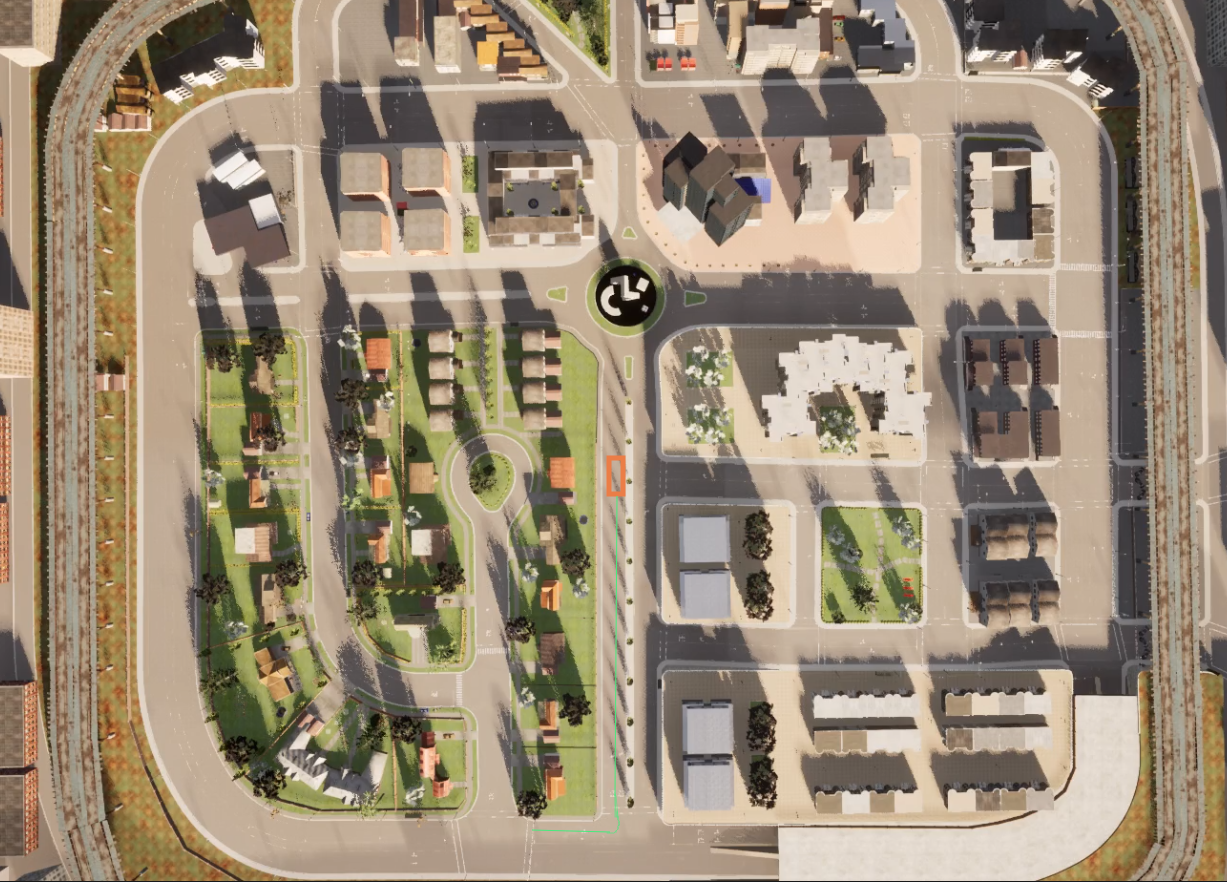
\includegraphics[height=0.6\textwidth]{images/Scenario.png}
        \caption{Scenario used in evaluation}
        \label{fig:Scenario}
    \end{figure}
    \begin{figure}[h] 
        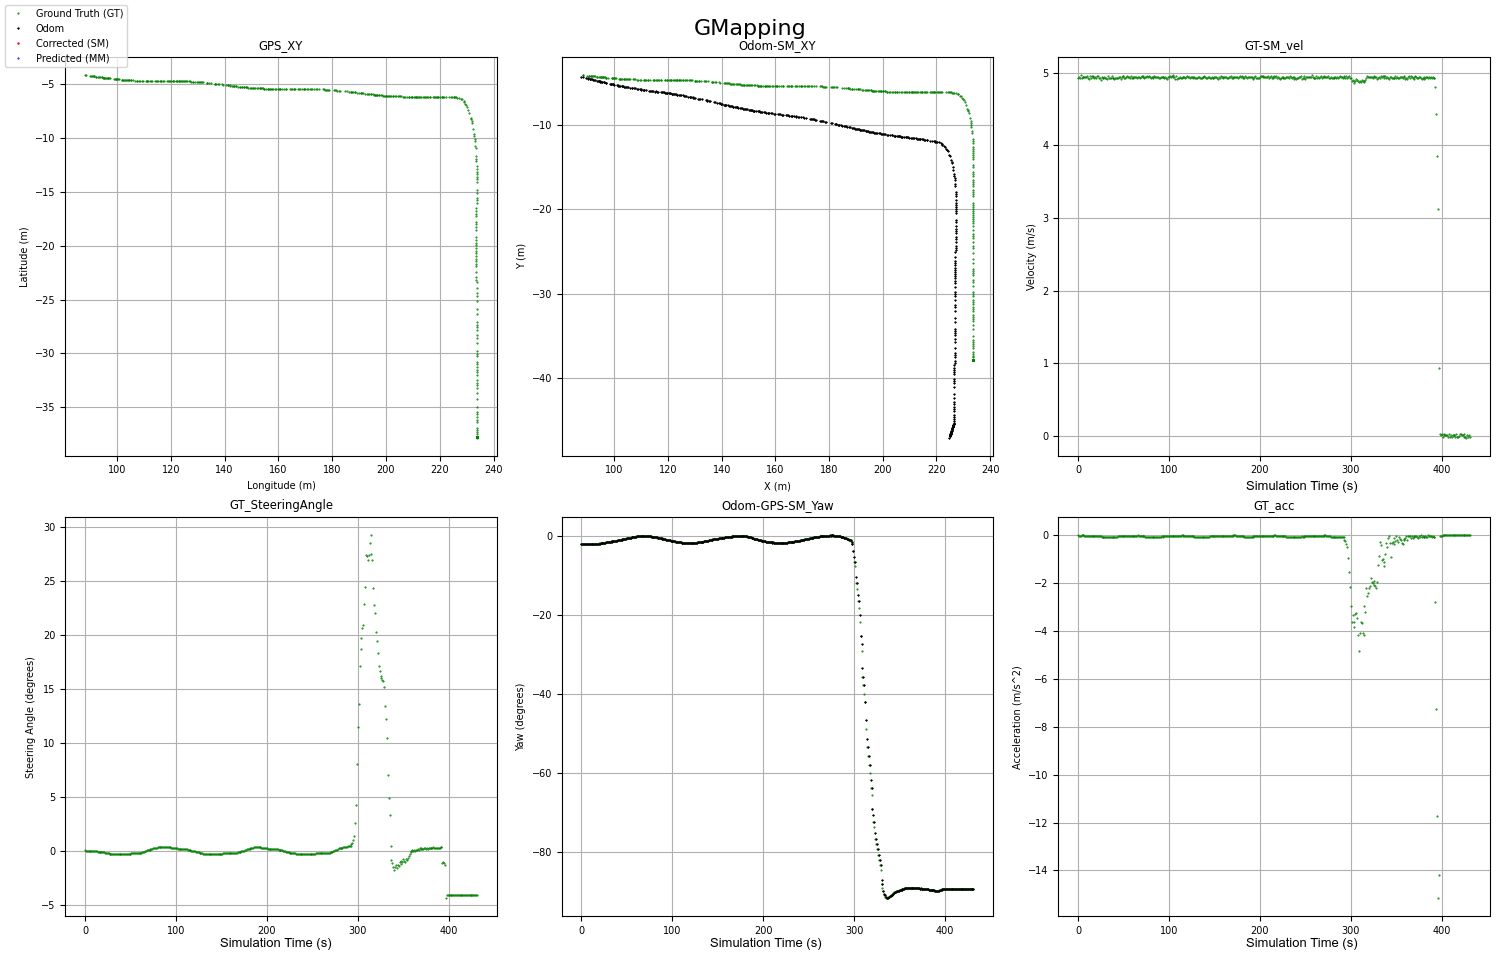
\includegraphics[height=0.6\textwidth]{images/GroundTruthParameters.png}
        \caption{Ground truth from GNSS and Odometry}
        \label{fig:GT_param}
    \end{figure}
    \begin{figure}[h] 
        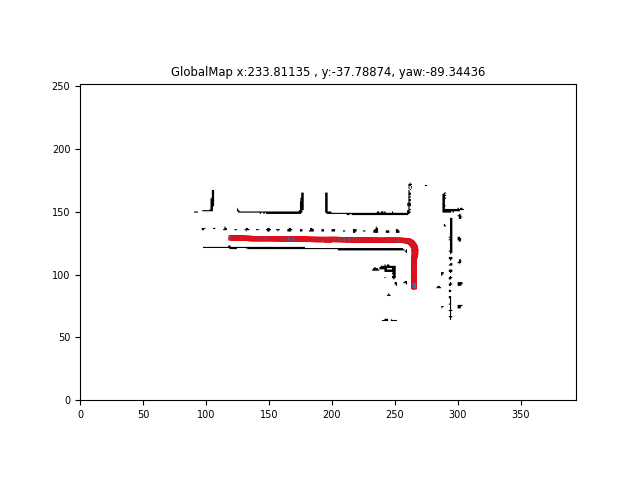
\includegraphics[height=0.6\textwidth]{images/GroundTruthMap.png}
        \caption{Map generated from GPS(ground truth)}
        \label{fig:GT_MAP}
    \end{figure}
The map generated from GPS is shown in \ref{fig:GT_MAP}
Since the odometry data from CARLA is noiseless and drift free, noise (Gaussian 0.1) and drift (modeled as a ramp function with slope 0.1) are manually added to the recorded data. The raw pose information obtained from GNSS sensor are in real coordinates in degrees, that is later converted to Cartesian coordinate system. The ground truth for the orientation is obtained from Inertial Measurement Unit (IMU). The signals velocity$(m/s)$, acceleration$(m/s^2)$ and steering angle$(degrees)$ are obtained from vehicle status message. The algorithm contains many tuning parameters that could be used for tuning and experimenting the results. However tuning parameters such as odometry noise and slope  would not be efficient as the scan matching algorithm could possibly reject its effect because of the error threshold parameter.
\clearpage
\par
LiDAR sensor mounted on the simulated car is noisy and finding the correct alignment using the scan matching algorithms usually provide results with residual error which provides confidence on how valid the results of the scan matching could be. Based on the residual error the particle filter decides if the correction step can be calculated with the scan matching results. In other words, If the scan matching error is more than a predefined threshold, the correction step is skipped and only prediction step is used to update the particle information.
Hence different thresholds of the error for scan matching algorithms discussed in the previous chapter is used in evaluating the implemented algorithms. 
\par
In case of GMapping, the particles are used to describe the posterior density $p(x_t, m | z_{1:t}, u_{0:t-1})$. Therefore to get an accurate estimate of pose and map, the posterior density has to be calculated precisely. Intuitively with more number of particles the posterior density can be estimated accurate. Hence the number of particles is also considered as a parameter that is tuned in order to evaluate the implemented algorithms. However this has effects on the computation efficiency leading to more computational resources and time.
\par
Apart from the metrics proposed in \cite{kuemmerle09auro},Run time of the algorithms is also compared. The algorithm runs with parallel processing ensuring efficient utilisation of the compute power. The evaluation is run on a workbench equipped with AMD Ryzen 7 4800H 2,9GHz processor and 16GB RAM. The cumulative comparison is provided in \ref{ssec:overallanalysis}.

\subsection{Evaluating SVD based ICP}
The evaluation of algorithms performed with error threshold set to 0.0015 and  0.001 along with particle count 20 and 50 are presented in below figures. It can be observed that with tighter thresholds, where the erroneous scan matching results are neglected, performs better. With more number of particles the final pose values are close to ground truth GPS data.
With lenient error threshold(0.0015) and less number of particles(20), a offset can be observed in the pose and orientation estimation\ref{fig:SVD_20_0.0015}. It can also be seen that difference in the pose and orientation estimation to the ground truth is never converging \ref{fig:SVD_20_0.0015_diff}
    \begin{figure}[h] 
        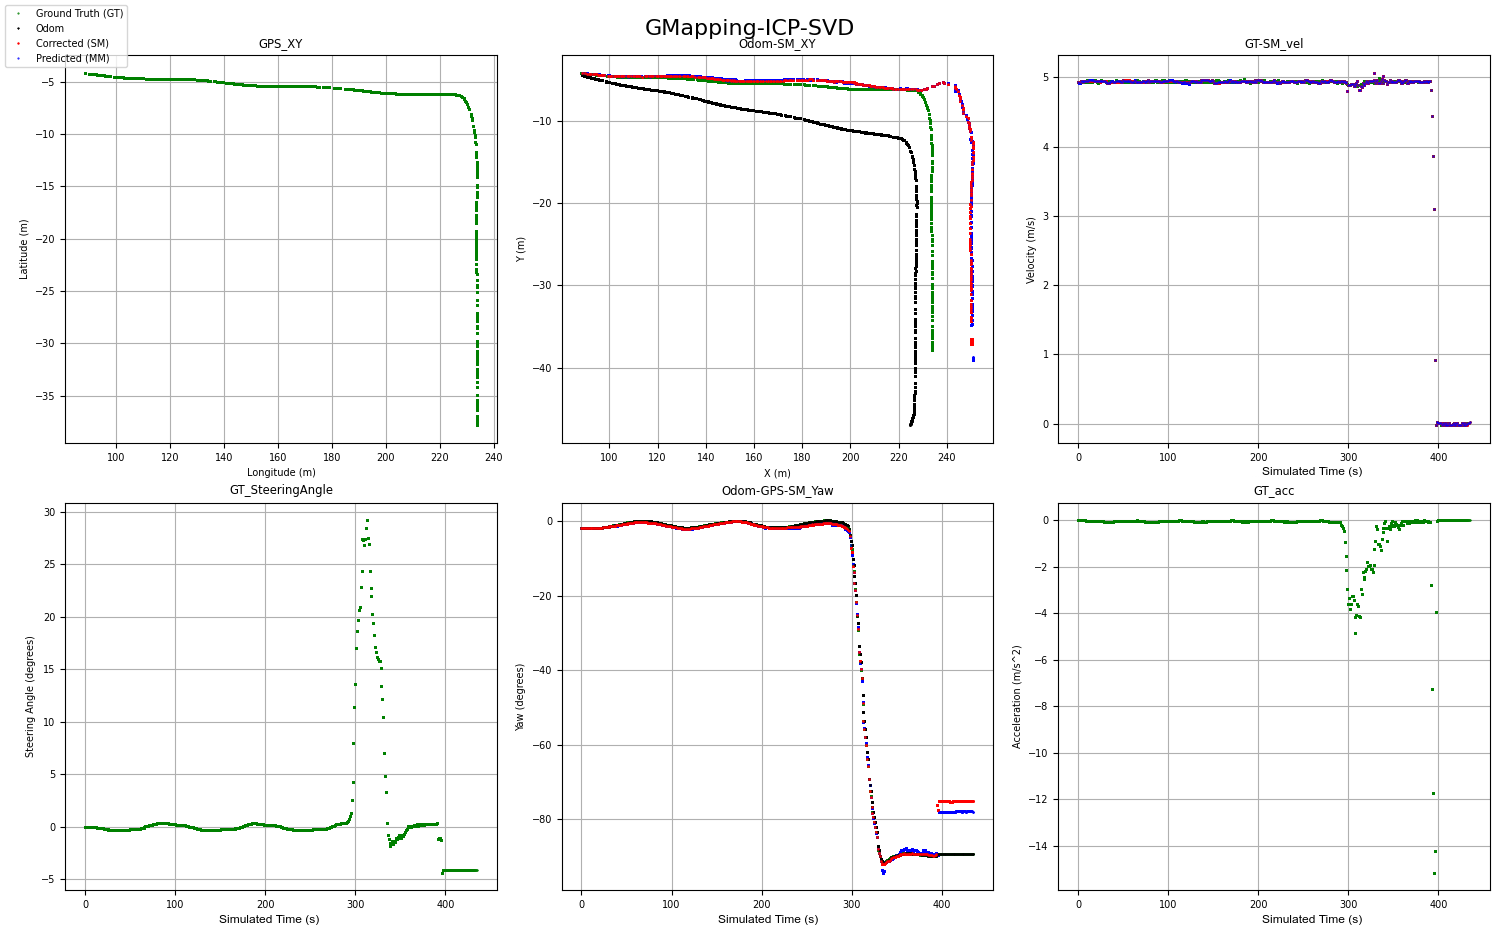
\includegraphics[height=0.6\textwidth]{images/GMapping-ICP-SVD_Map_20_0.0015.png}
        \caption{SVD based ICP- Particles(20), Error Threshold(0.0015)}
        \label{fig:SVD_20_0.0015}
    \end{figure}
    \begin{figure}[h] 
        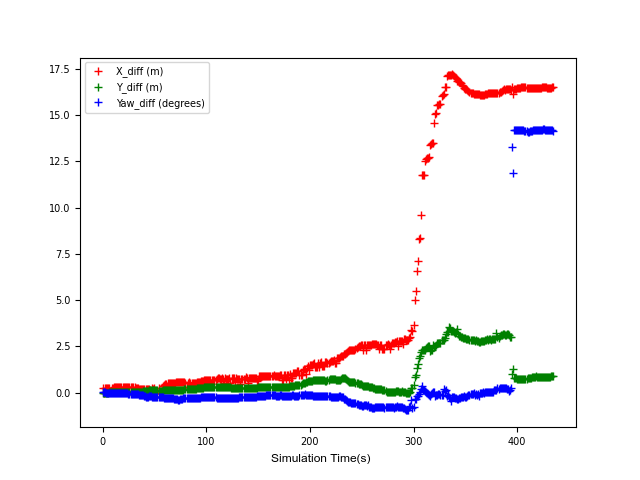
\includegraphics[height=0.4\textwidth]{images/GMapping-ICP-SVD_True_vs_Crct_20_0.0015.png}
        \caption{SVD based ICP- Difference between ground truth(GPS) and estimation}
        \label{fig:SVD_20_0.0015_diff}
    \end{figure}
\clearpage
Just increasing the number of particles to 50, provides marginally better results than the previous case \ref{fig:SVD_50_0.0015}, \ref{fig:SVD_50_0.0015_diff}
    \begin{figure}[h] 
        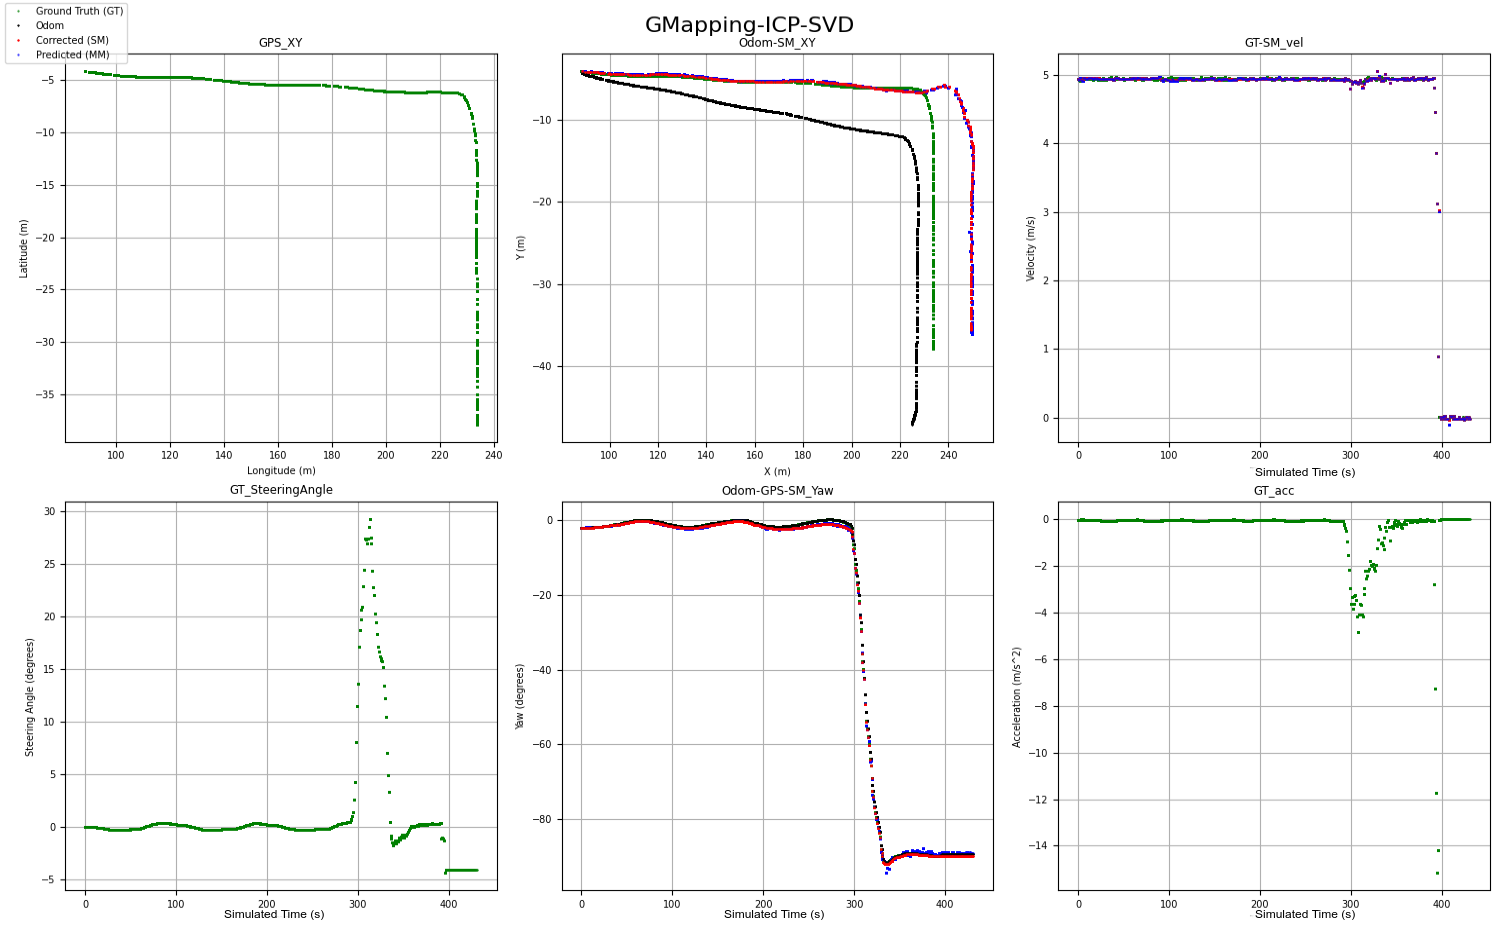
\includegraphics[height=0.6\textwidth]{images/GMapping-ICP-SVD_Map_50_0.0015.png}
        \caption{SVD based ICP- Particles(50), Error Threshold(0.0015)}
        \label{fig:SVD_50_0.0015}
    \end{figure}
    \begin{figure}[h]
        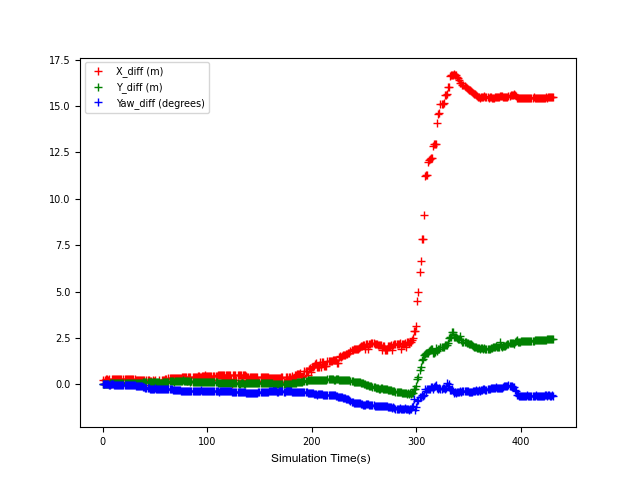
\includegraphics[height=0.4\textwidth]{images/GMapping-ICP-SVD_True_vs_Crct_50_0.0015.png}
        \caption{SVD based ICP- Difference between ground truth(GPS) and estimation}
        \label{fig:SVD_50_0.0015_diff}
    \end{figure}
\clearpage
However with tighter error threshold(0.001) the performance of the system is better, with pose more aligned to the ground truth \ref{fig:SVD_20_0.001}, \ref{fig:SVD_20_0.001_diff}.
    \begin{figure}[h] 
        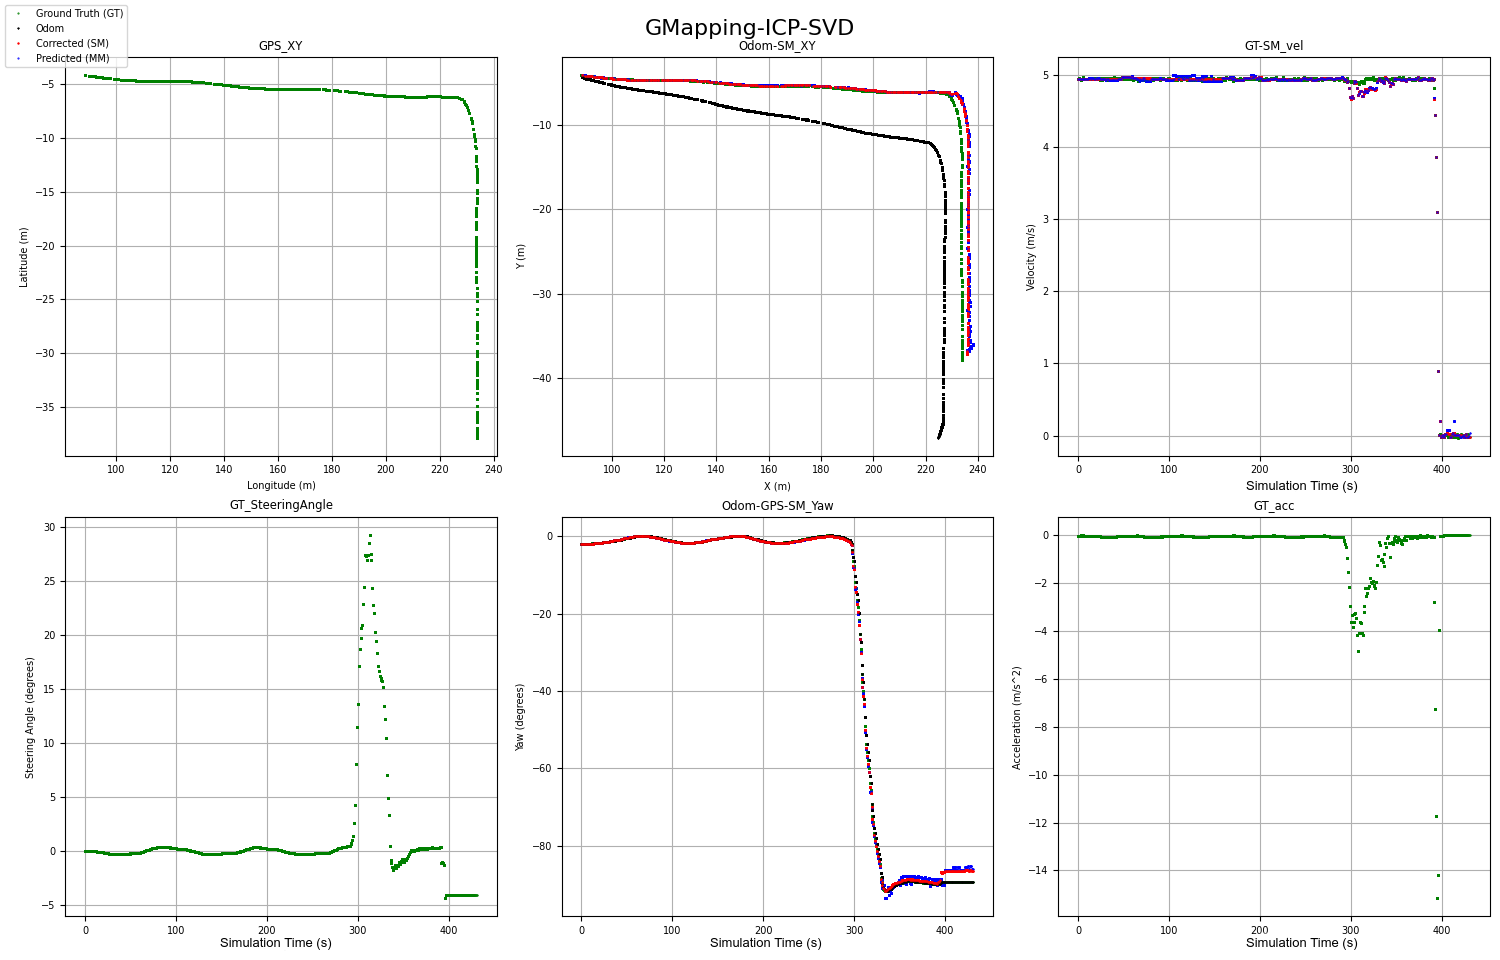
\includegraphics[height=0.6\textwidth]{images/GMapping-ICP-SVD_Map_20_0.001.png}
        \caption{SVD based ICP- Particles(20), Error Threshold(0.001)}
        \label{fig:SVD_20_0.001}
    \end{figure}
    \begin{figure}[h] 
        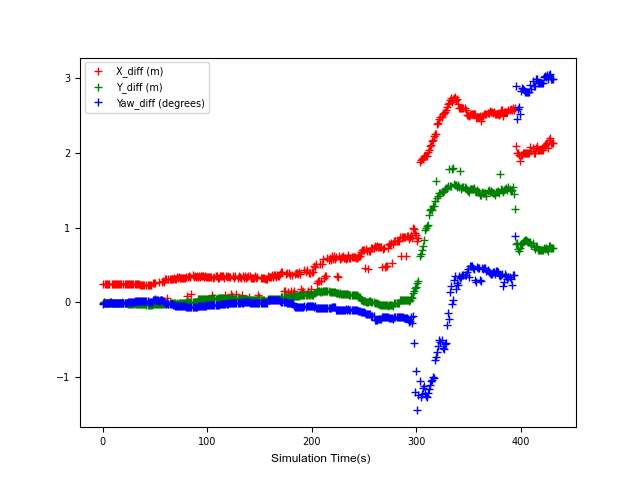
\includegraphics[height=0.4\textwidth]{images/GMapping-ICP-SVD_True_vs_Crct_20_0.001.png}
        \caption{SVD based ICP- Difference between ground truth(GPS) and estimation}
        \label{fig:SVD_20_0.001_diff}
    \end{figure}
\clearpage
With more number of particles, the results are even better \ref{fig:SVD_50_0.001}, \ref{fig:SVD_50_0.001_diff}
    \begin{figure}[h] 
        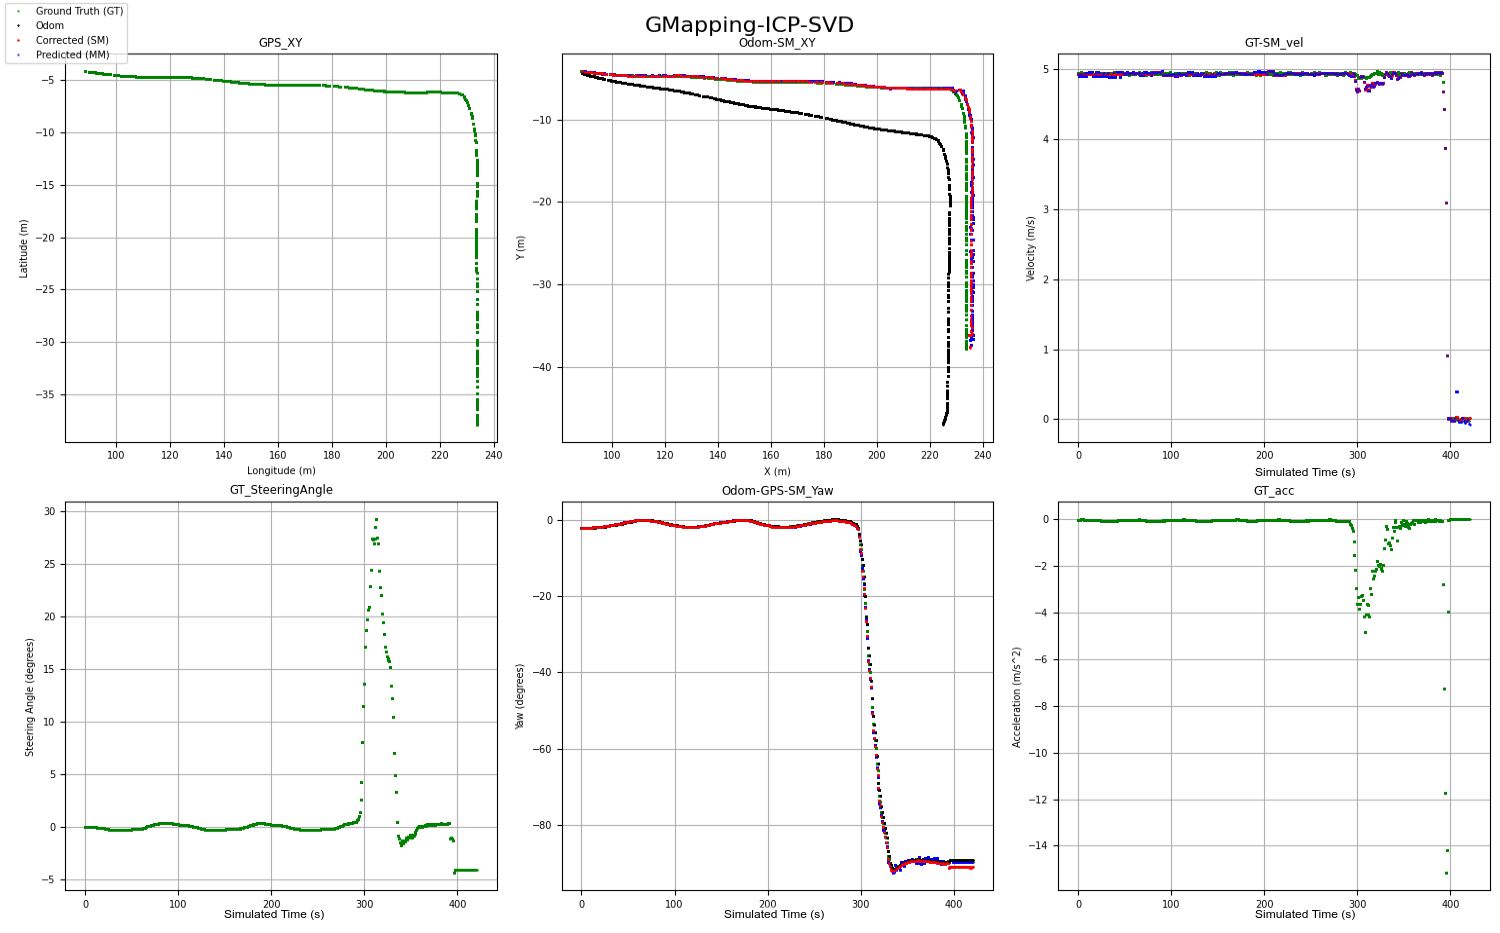
\includegraphics[height=0.6\textwidth]{images/GMapping-ICP-SVD_Map_50_0.001.png}
        \caption{SVD based ICP- Particles(50), Error Threshold(0.001)}
        \label{fig:SVD_50_0.001}
    \end{figure}
    \begin{figure}[h] 
        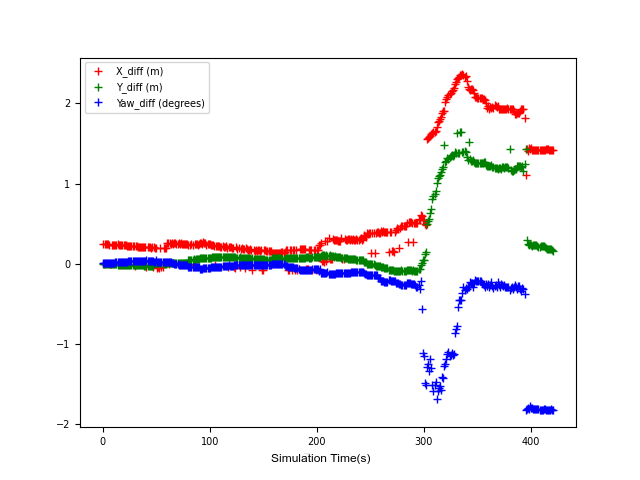
\includegraphics[height=0.4\textwidth]{images/GMapping-ICP-SVD_True_vs_Crct_50_0.001.png}
        \caption{SVD based ICP- Difference between ground truth(GPS) and estimation}
        \label{fig:SVD_50_0.001_diff}
    \end{figure}
\clearpage

\subsection{Evaluating LS based ICP}
The evaluation of algorithms performed with error threshold set to 0.0025 and  0.002 along with particle count 20 and 50 are presented in below figures. It can be observed that with tighter thresholds, where the erroneous scan matching results are neglected, performs better. With more number of particles the final pose values are close to ground truth GPS data.
With lenient error threshold(0.0025) and less number of particles(20), a offset can be observed in the pose and orientation estimation\ref{fig:LS_20_0.0025}. Like in the case of SVD based ICP, It can also be seen that difference in the pose and orientation estimation to the ground truth is never converging \ref{fig:LS_20_0.0025_diff}.
    \begin{figure}[h] 
        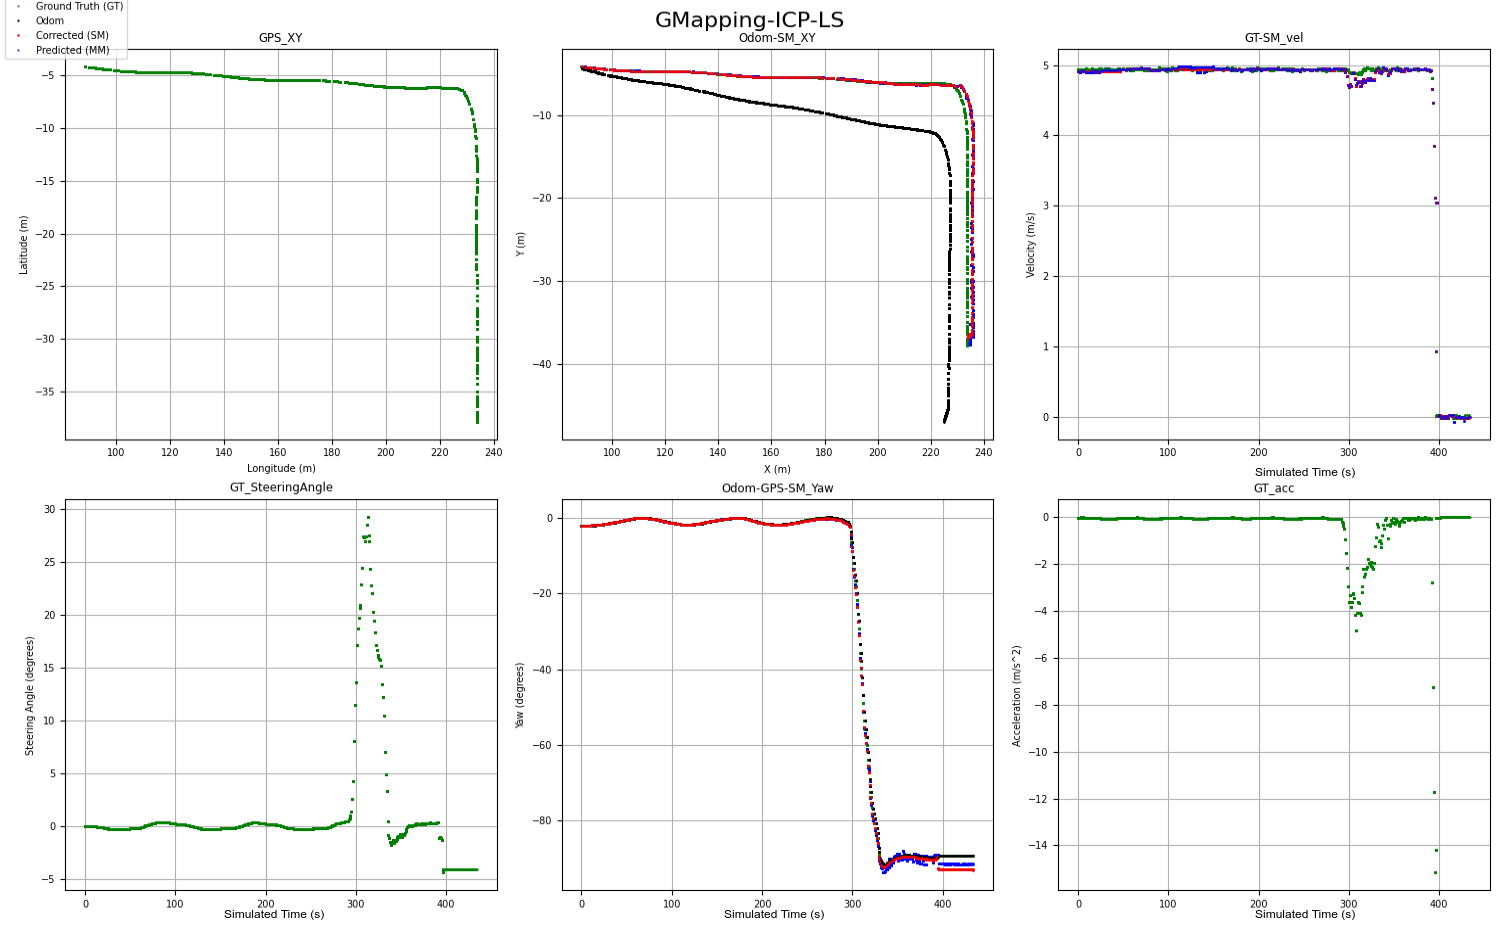
\includegraphics[height=0.6\textwidth]{images/GMapping-ICP-LS_Map_20_0.0025.png}
        \caption{LS based ICP- Particles(20), Error Threshold(0.0025)}
        \label{fig:LS_20_0.0025}
    \end{figure}
    \begin{figure}[h] 
        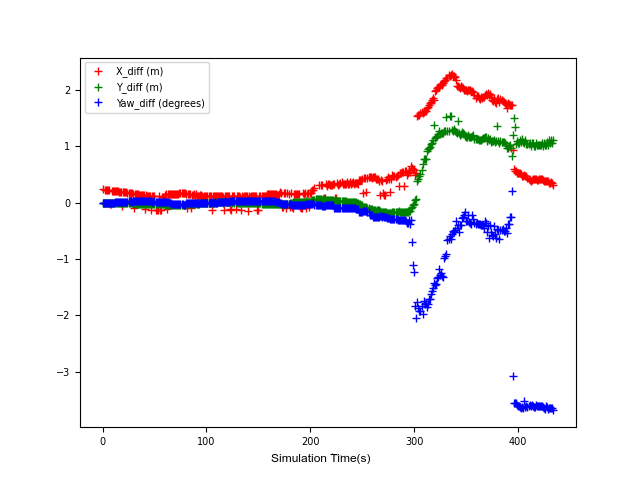
\includegraphics[height=0.4\textwidth]{images/GMapping-ICP-LS_True_vs_Crct_20_0.0025.png}
        \caption{LS based ICP- Difference between ground truth(GPS) and estimation}
        \label{fig:LS_20_0.0025_diff}
    \end{figure}
\clearpage
Just increasing the number of particles to 50, provides marginally better results than the previous case \ref{fig:LS_50_0.0025}, \ref{fig:LS_50_0.0025_diff}.
    \begin{figure}[h] 
        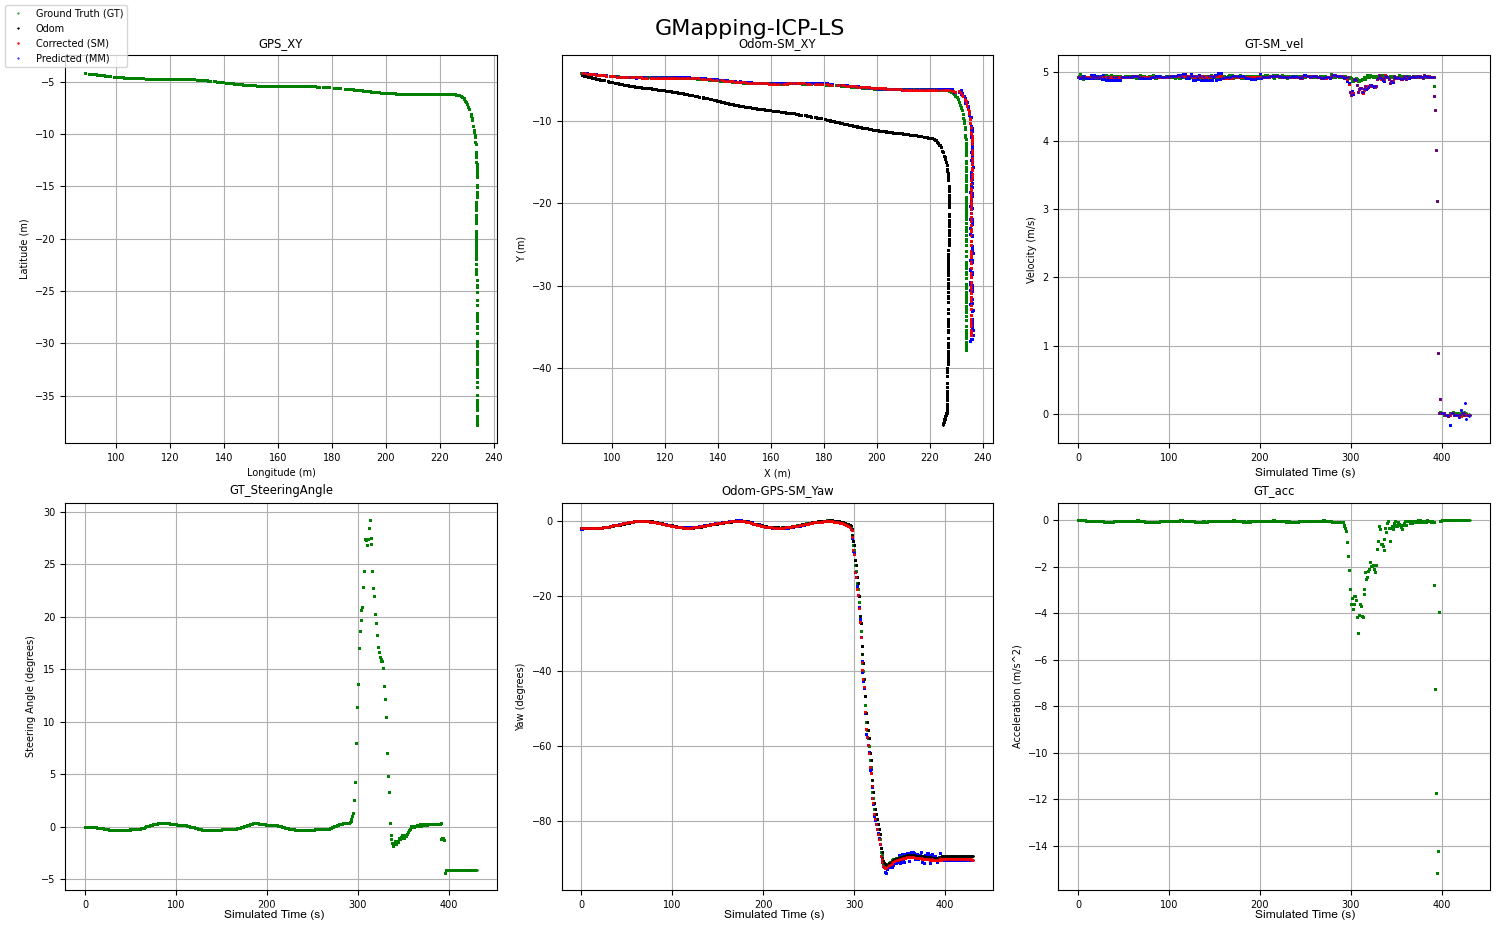
\includegraphics[height=0.6\textwidth]{images/GMapping-ICP-LS_Map_50_0.0025.png}
        \caption{LS based ICP- Particles(50), Error Threshold(0.0025)}
        \label{fig:LS_50_0.0025}
    \end{figure}
    \begin{figure}[h] 
        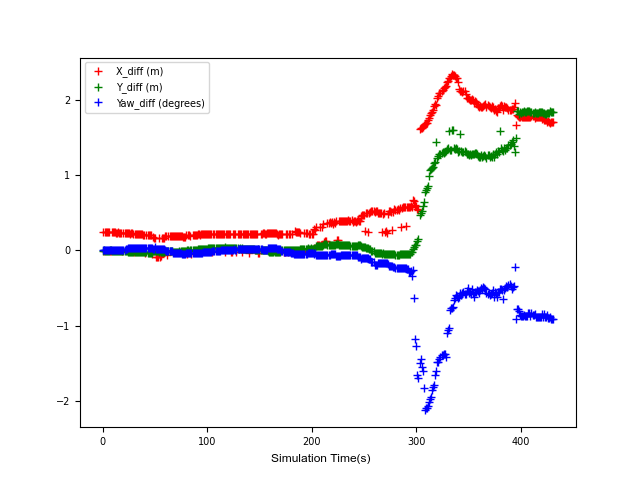
\includegraphics[height=0.4\textwidth]{images/GMapping-ICP-LS_True_vs_Crct_50_0.0025.png}
        \caption{LS based ICP- Difference between ground truth(GPS) and estimation}
        \label{fig:LS_50_0.0025_diff}
    \end{figure}
\clearpage
However with tighter error threshold(0.002) the performance of the system is better, with pose more aligned to the ground truth \ref{fig:LS_20_0.002}, \ref{fig:LS_20_0.002_diff}.
    \begin{figure}[h] 
        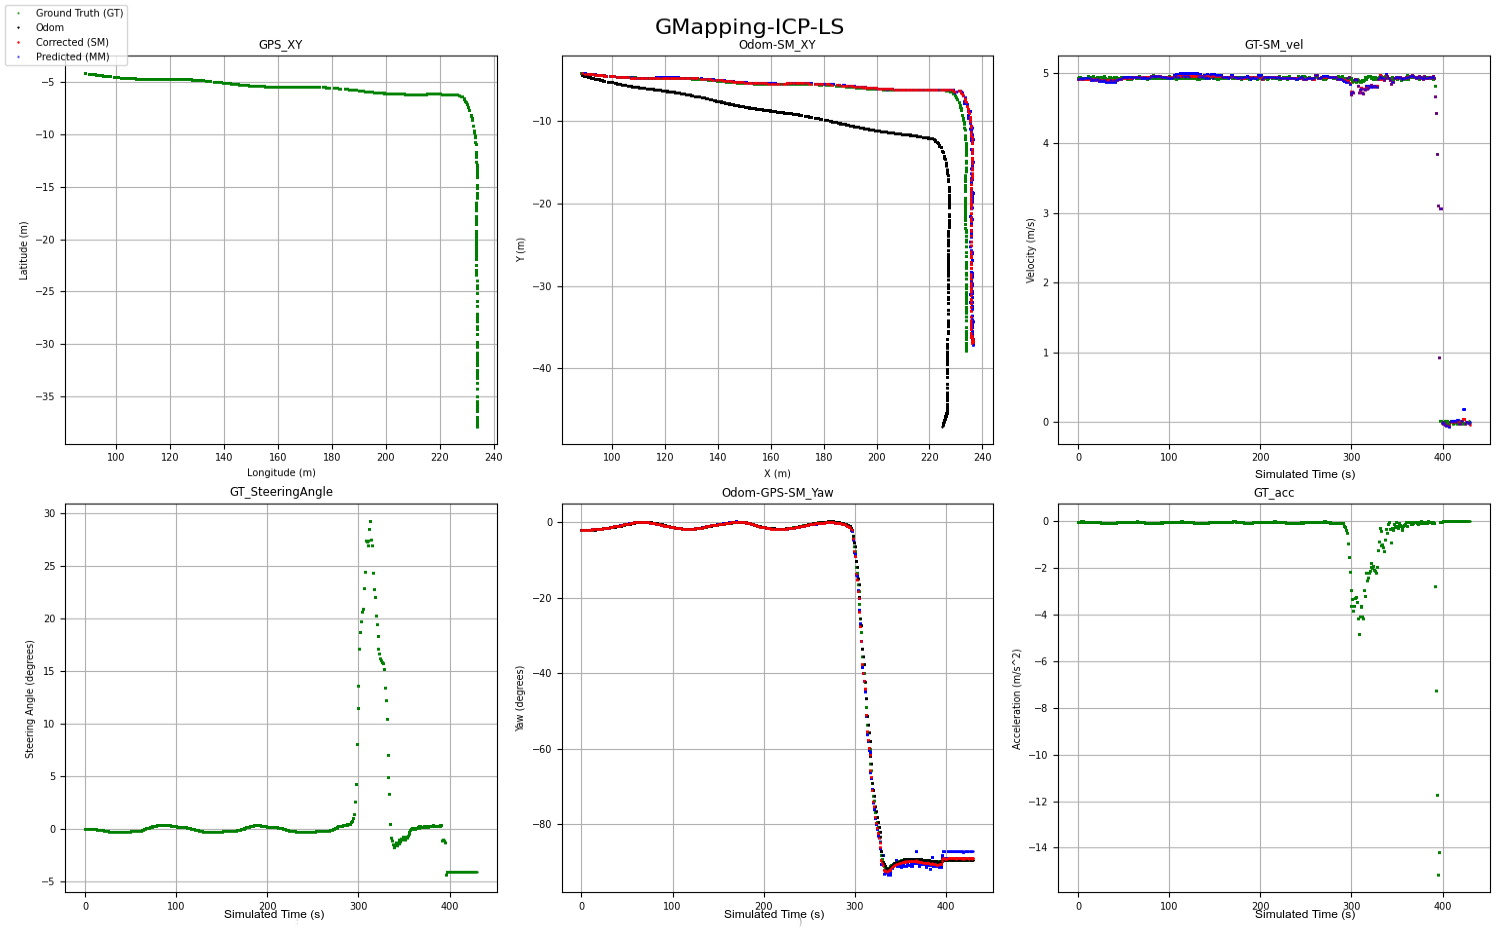
\includegraphics[height=0.6\textwidth]{images/GMapping-ICP-LS_Map_20_0.002.png}
        \caption{LS based ICP- Particles(20), Error Threshold(0.002)}
        \label{fig:LS_20_0.002}
    \end{figure}
    \begin{figure}[h] 
        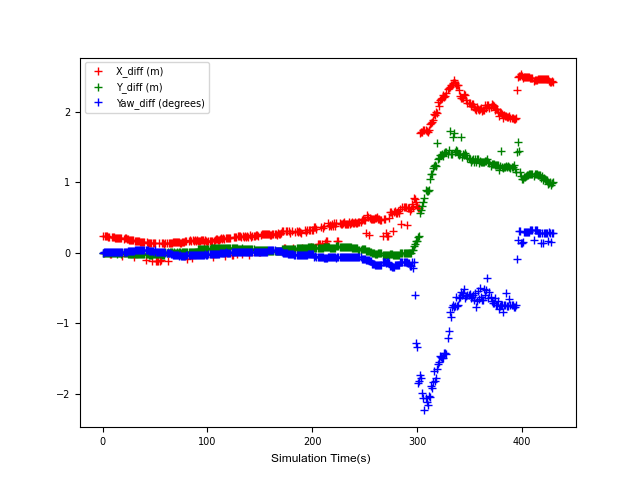
\includegraphics[height=0.4\textwidth]{images/GMapping-ICP-LS_True_vs_Crct_20_0.002.png}
        \caption{LS based ICP- Difference between ground truth(GPS) and estimation}
        \label{fig:LS_20_0.002_diff}
    \end{figure}
\clearpage
With more number of particles, the results are even better \ref{fig:LS_50_0.002}, \ref{fig:LS_50_0.002_diff}.
    \begin{figure}[h] 
        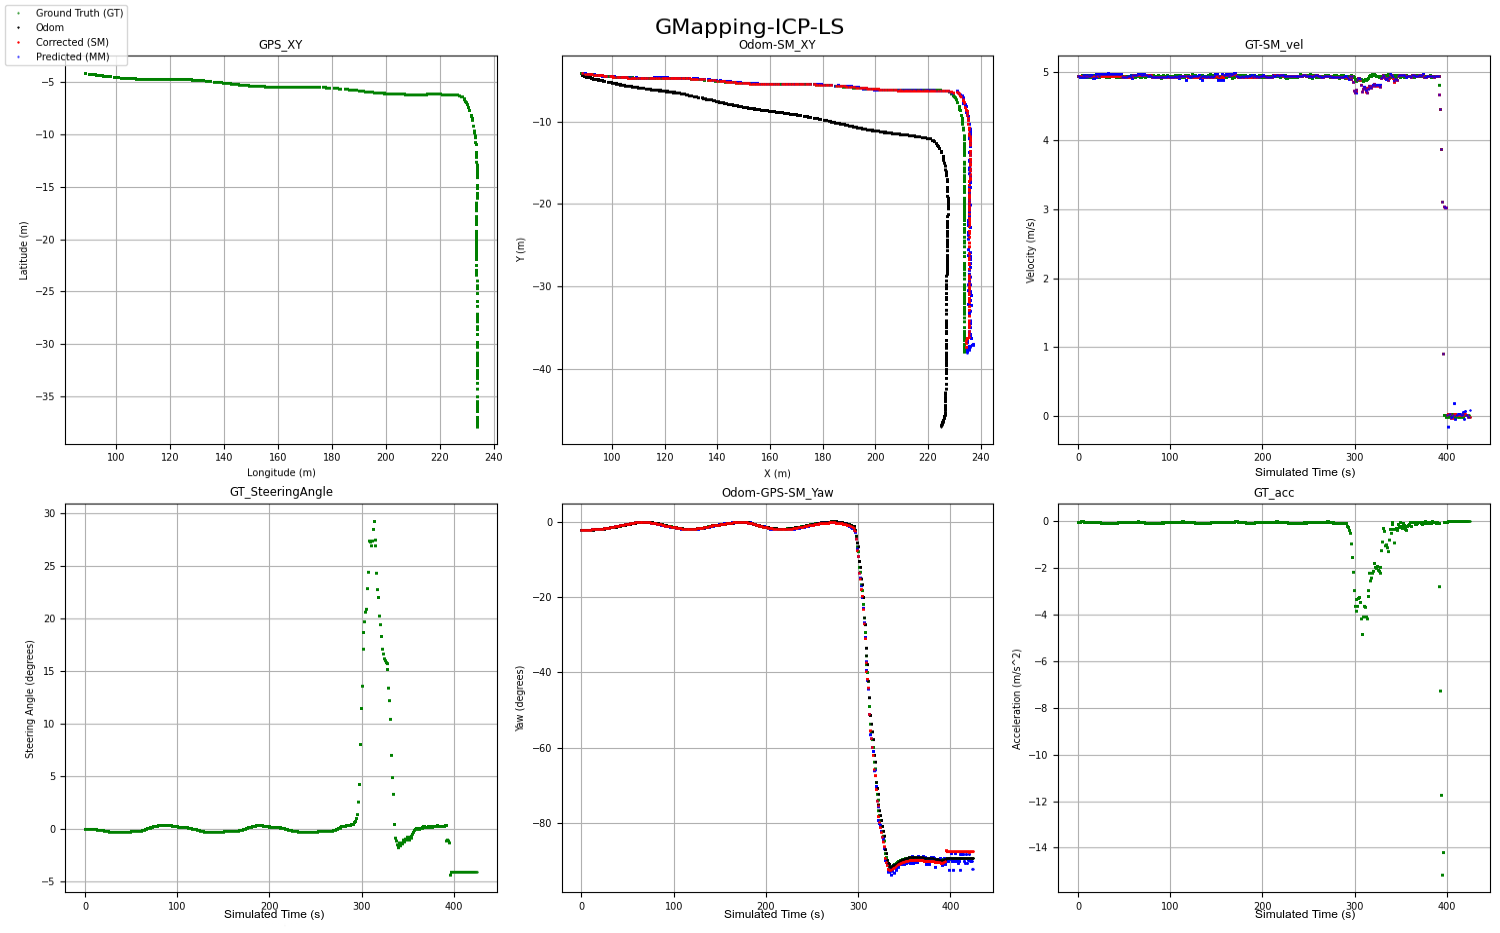
\includegraphics[height=0.6\textwidth]{images/GMapping-ICP-LS_Map_50_0.002.png}
        \caption{LS based ICP- Particles(50), Error Threshold(0.002)}
        \label{fig:LS_50_0.002}
    \end{figure}
    \begin{figure}[h] 
        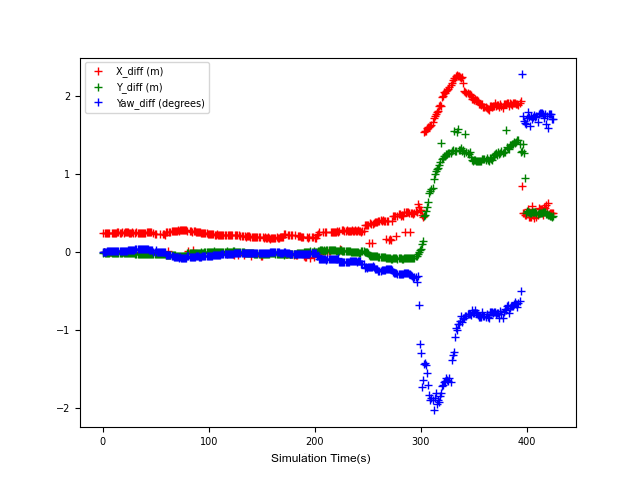
\includegraphics[height=0.4\textwidth]{images/GMapping-ICP-LS_True_vs_Crct_50_0.002.png}
        \caption{LS based ICP- Difference between ground truth(GPS) and estimation}
        \label{fig:LS_50_0.002_diff}
    \end{figure}
\clearpage

\subsection{Evaluating RTCSM}
Unlike ICP, RTCSM does not have a error threshold but has a confidence to how good the scan matching results are. In the RTCSM algorithm, local map created from the previous pose update is correlated with the local map created from the present particle position. In this process a Gaussian(possible pose estimate as a mask) is placed over every single occupied cell for every possible orientation. The confidence value is calculated that is used as a criteria for acceptance. Similar to ICP, the evaluation is repeated for four possible combinations of particle count (20 and 50) and confidence values (0.052 and 0.05). The increasing difference at the last few seconds in the longitudinal direction is observed in all the following cases because of wrong velocity estimation hence it is not considered in analysis further.
With lower confidence(0.05) and less number of particles(20), a offset can be observed in the pose and orientation estimation \ref{fig:RTCSM_20_0.05}. Like in the case of ICP, It can also be seen that difference in the pose and orientation estimation to the ground truth is never converging \ref{fig:RTCSM_20_0.05_diff}.
    \begin{figure}[h] 
        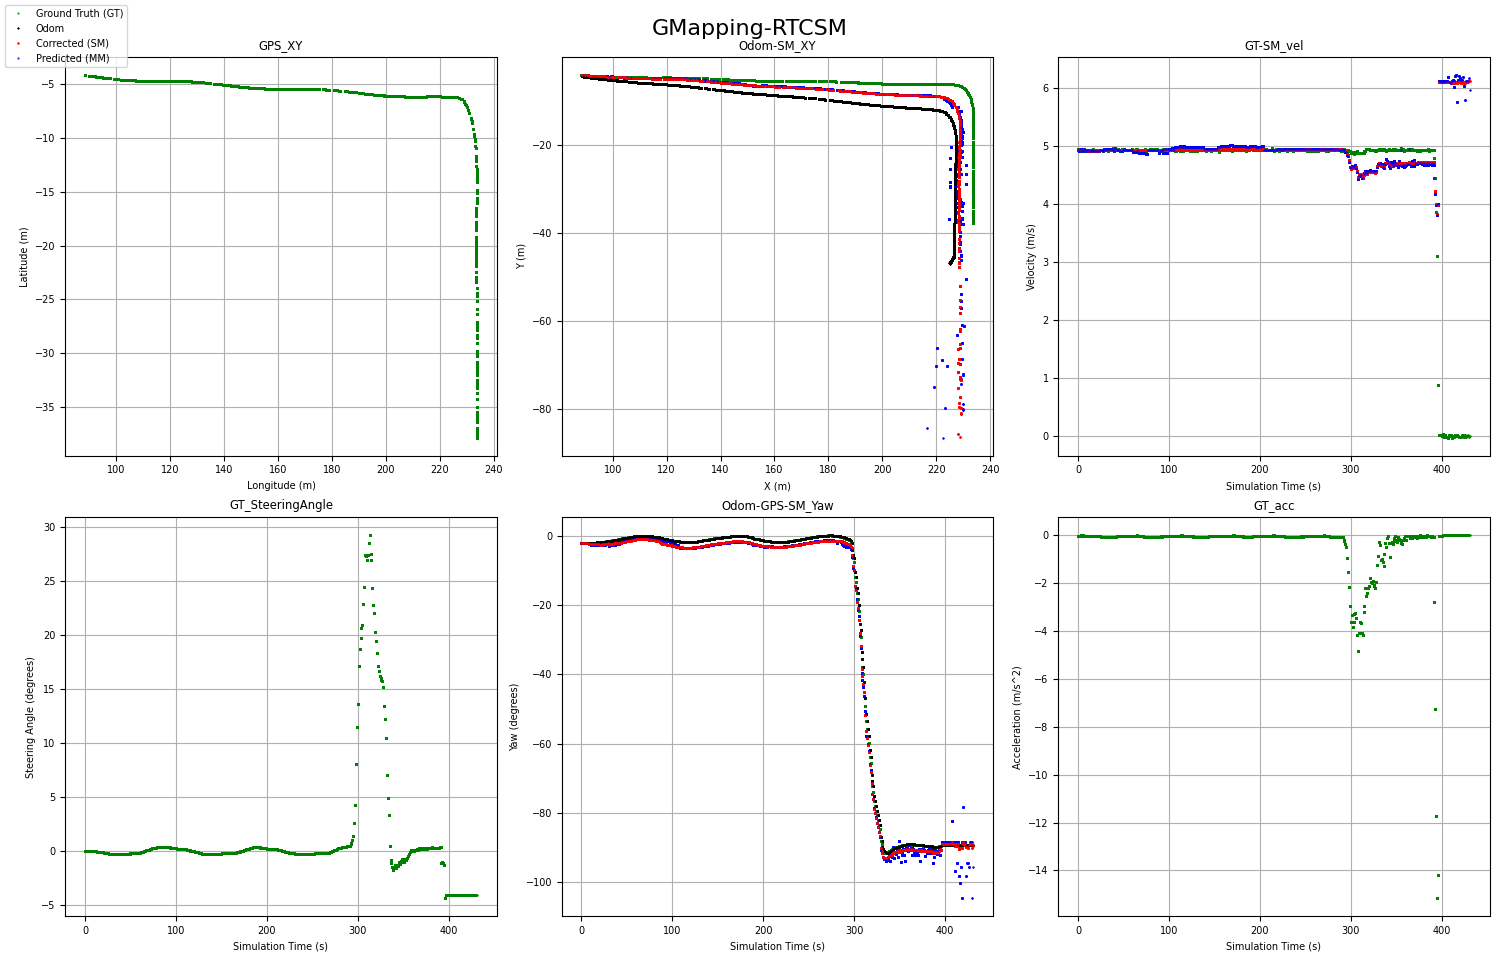
\includegraphics[height=0.6\textwidth]{images/GMapping-RTCSM_Map_20_0.05.png}
        \caption{RTCSM- Particles(20), Error Threshold(0.05)}
        \label{fig:RTCSM_20_0.05}
    \end{figure}
    \begin{figure}[h] 
        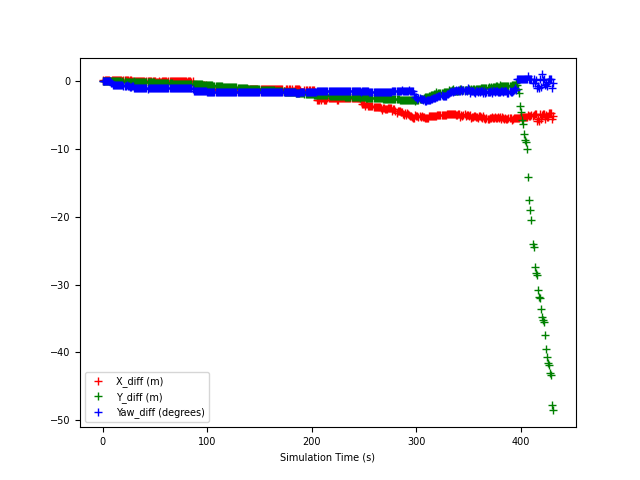
\includegraphics[height=0.4\textwidth]{images/GMapping-RTCSM_True_vs_Crct_20_0.05.png}
        \caption{RTCSM- Difference between ground truth(GPS) and estimation}
        \label{fig:RTCSM_20_0.05_diff}
    \end{figure}
\clearpage
Just increasing the number of particles to 50, provides marginally better results than the previous case \ref{fig:RTCSM_50_0.05}, \ref{fig:RTCSM_50_0.05_diff}.
    \begin{figure}[h] 
        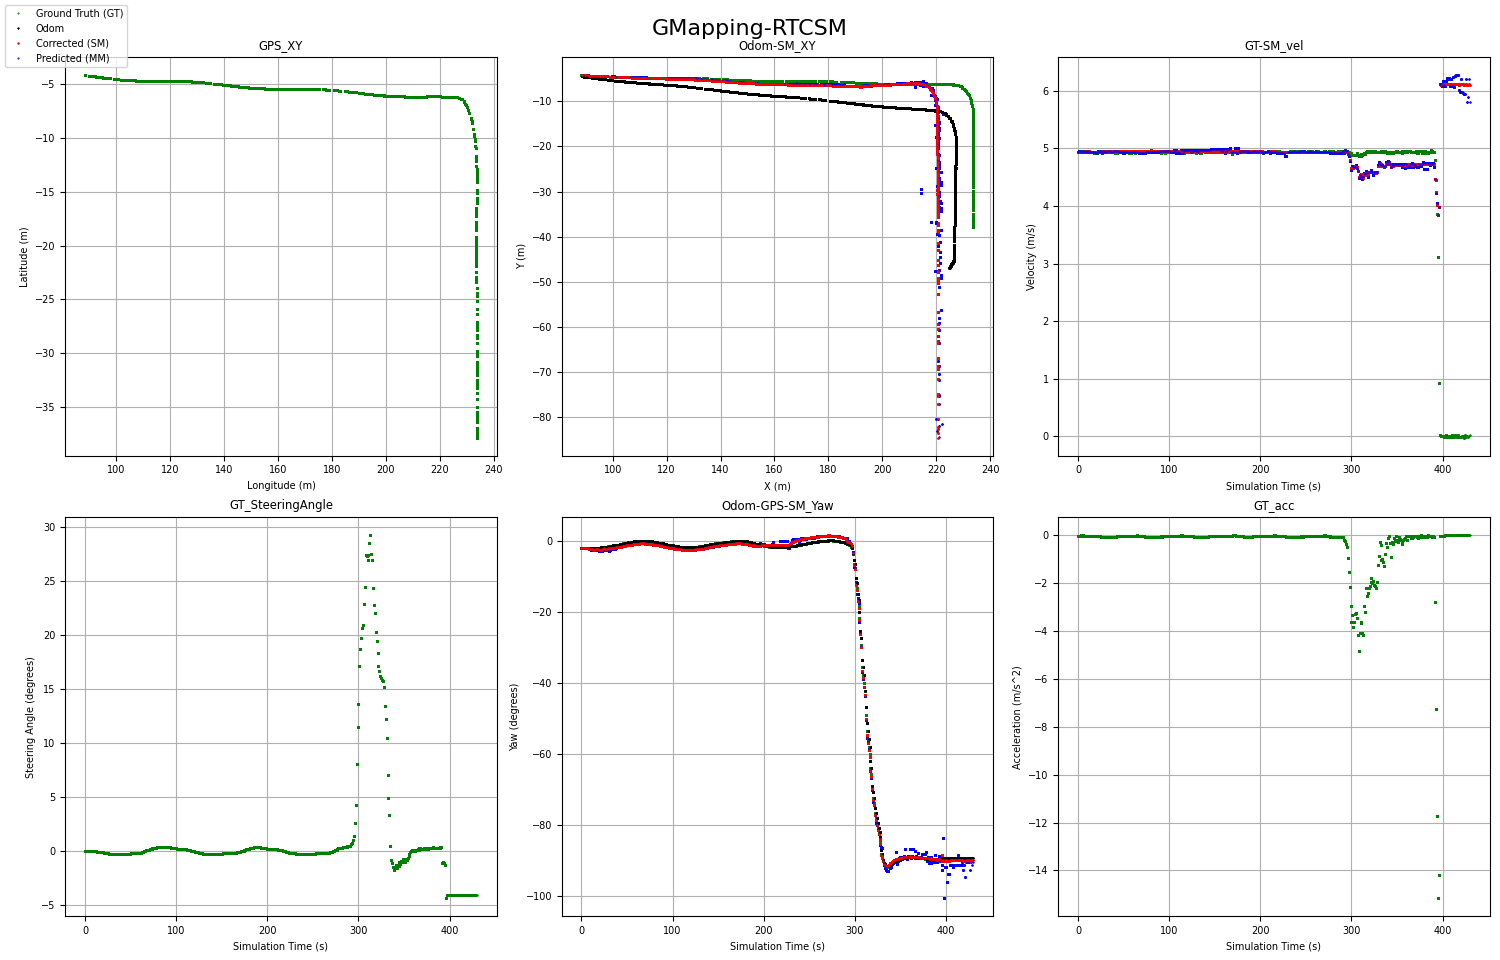
\includegraphics[height=0.6\textwidth]{images/GMapping-RTCSM_Map_50_0.05.png}
        \caption{RTCSM- Particles(50), Error Threshold(0.02)}
        \label{fig:RTCSM_50_0.05}
    \end{figure}
    \begin{figure}[h] 
        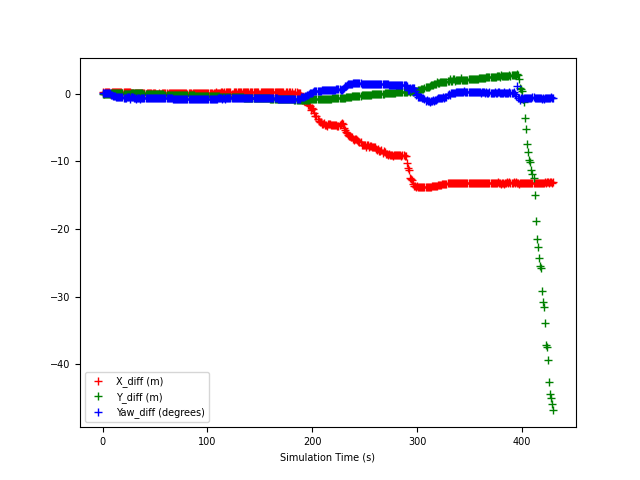
\includegraphics[height=0.4\textwidth]{images/GMapping-RTCSM_True_vs_Crct_50_0.05.png}
        \caption{RTCSM- Difference between ground truth(GPS) and estimation}
        \label{fig:RTCSM_50_0.05_diff}
    \end{figure}
\clearpage
However with higher confidence threshold(0.052) the performance of the system is better, with pose more aligned to the ground truth \ref{fig:RTCSM_20_0.052}, \ref{fig:RTCSM_20_0.052_diff}.
    \begin{figure}[h] 
        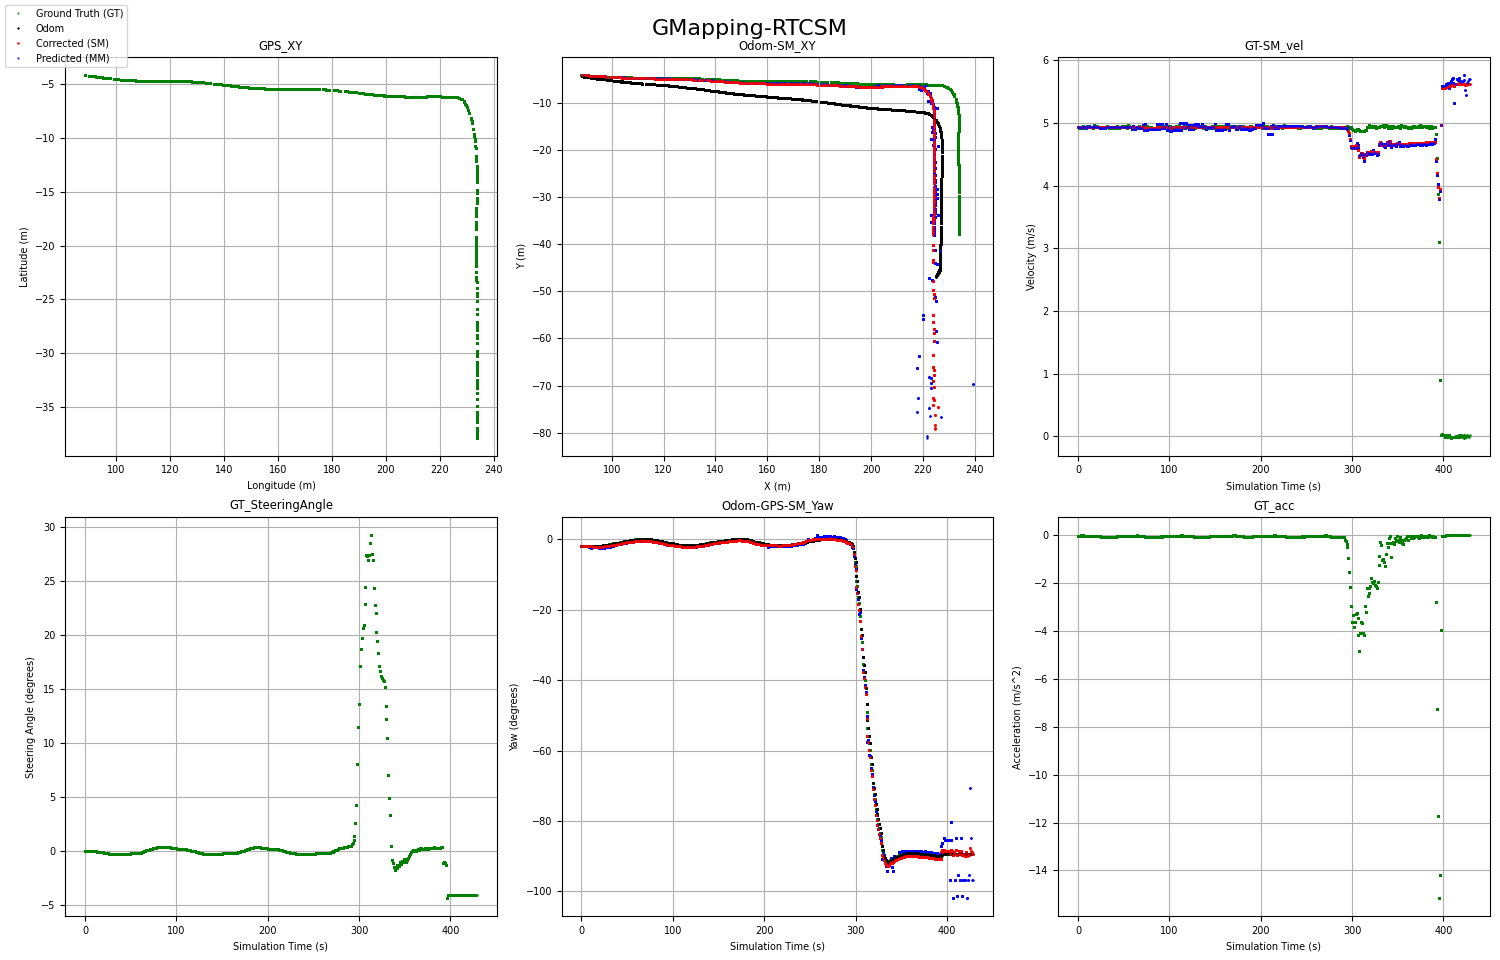
\includegraphics[height=0.6\textwidth]{images/GMapping-RTCSM_Map_20_0.052.png}
        \caption{RTCSM- Particles(20), Error Threshold(0.052)}
        \label{fig:RTCSM_20_0.052}
    \end{figure}
    \begin{figure}[h] 
        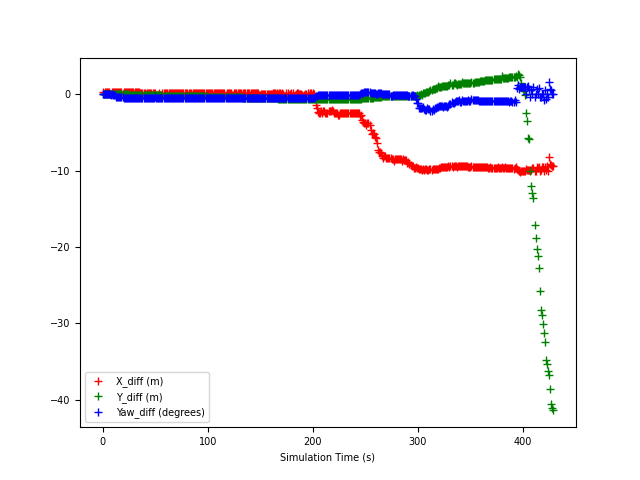
\includegraphics[height=0.4\textwidth]{images/GMapping-RTCSM_True_vs_Crct_20_0.052.png}
        \caption{RTCSM- Difference between ground truth(GPS) and estimation}
        \label{fig:RTCSM_20_0.052_diff}
    \end{figure}
\clearpage
With more number of particles, the results are even better \ref{fig:RTCSM_50_0.052}, \ref{fig:RTCSM_50_0.052_diff}.
    \begin{figure}[h] 
        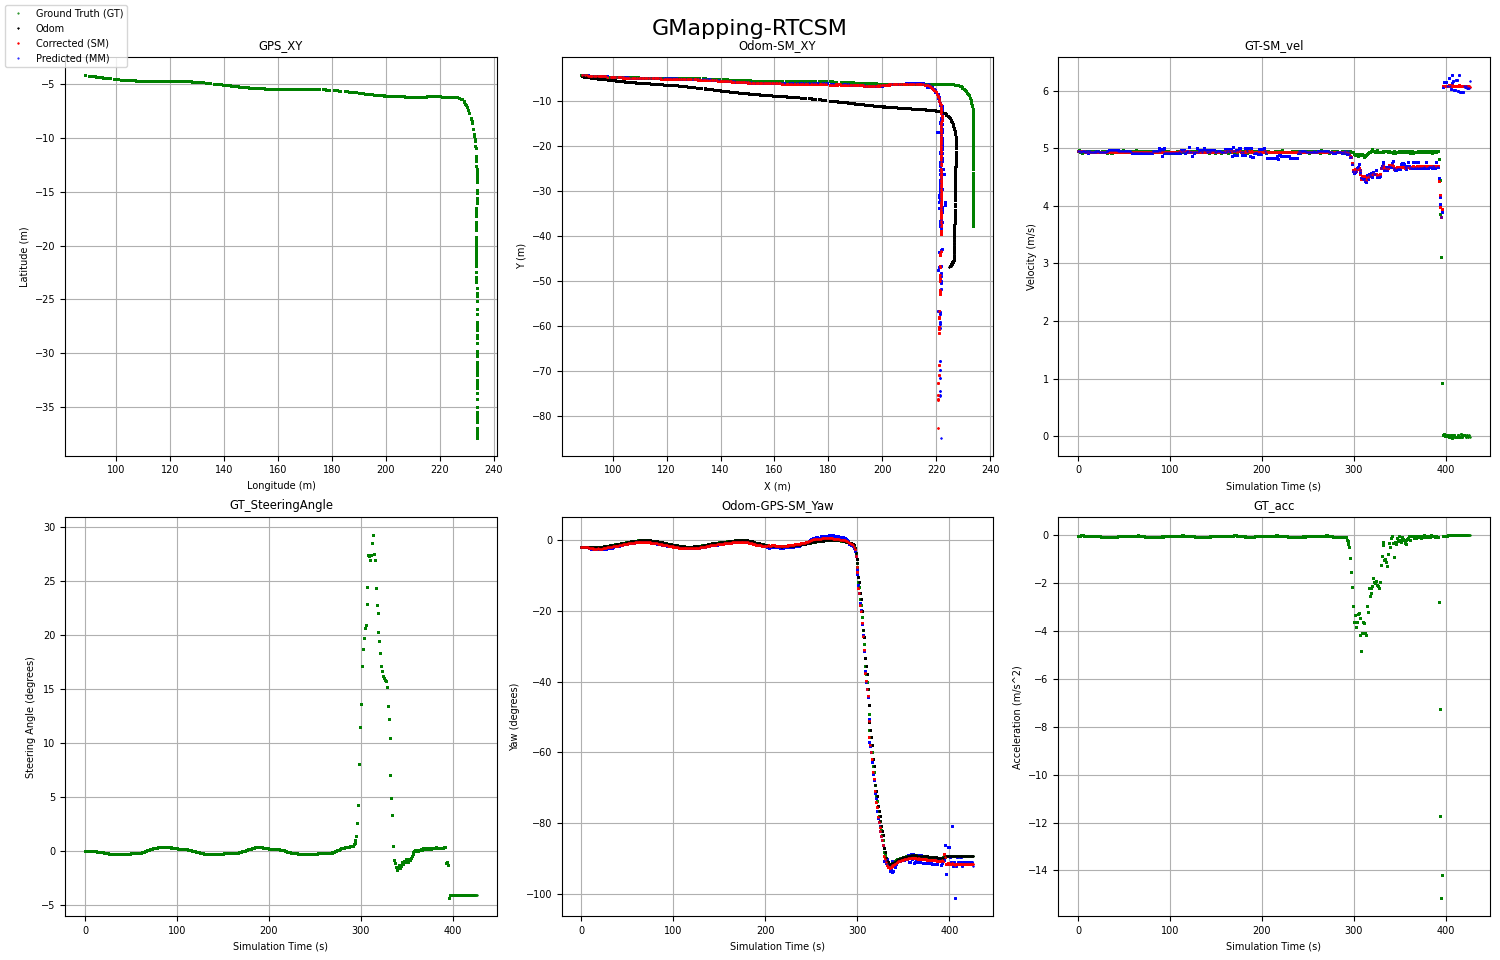
\includegraphics[height=0.6\textwidth]{images/GMapping-RTCSM_Map_50_0.052.png}
        \caption{RTCSM- Particles(50), Error Threshold(0.052)}
        \label{fig:RTCSM_50_0.052}
    \end{figure}
    \begin{figure}[h] 
        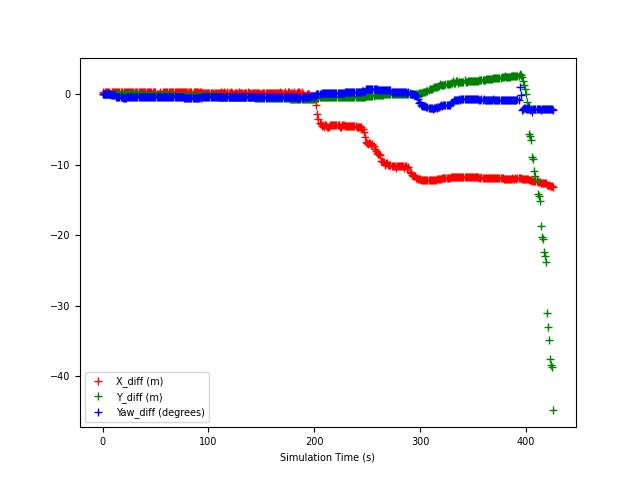
\includegraphics[height=0.4\textwidth]{images/GMapping-RTCSM_True_vs_Crct_50_0.052.png}
        \caption{RTCSM- Difference between ground truth(GPS) and estimation}
        \label{fig:RTCSM_50_0.052_diff}
    \end{figure}
\clearpage

\subsection{Overall analysis} \label{ssec:overallanalysis}
The benchmark parameters are calculated and summarised in the table below 
    \begin{figure}[h] 
        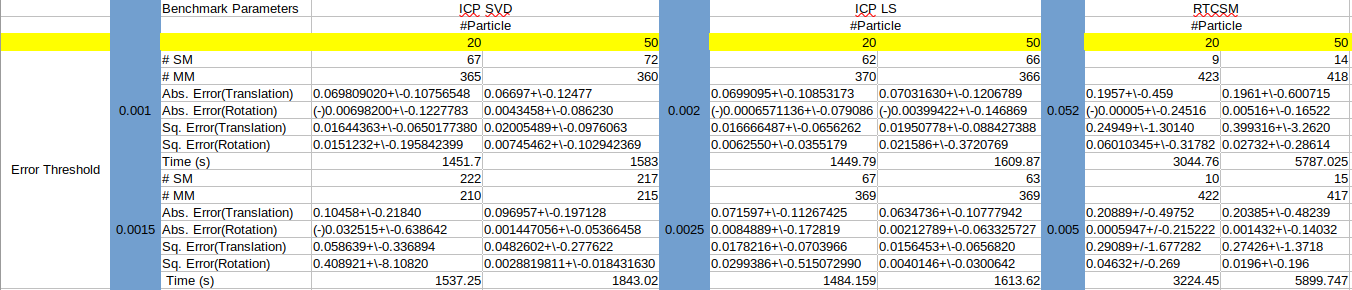
\includegraphics[width=1\textwidth]{images/Benchmark.png}
        \caption{Evaluation result of scan matching algorithms}
        \label{fig:benchmark}
    \end{figure}
In the figure \ref{fig:benchmark}, $#SM$ and $#MM$ denote the number of times scan matching and motion model had been taken into estimation respectively. It can be observed that ICP-LS and ICP-SVD have comparable results in terms of accuracy and computation time with a demanding threshold criteria. However in the case of a relaxed error threshold criteria, ICP-LS performs better. A strict criteria  for the error threshold forces the system to discard the scan matching result for a better map. As an effect the algorithm following it is not executed, resulting in particle states being updated with motion model prediction. 
Both absolute and squared error are considered in the evaluation, they are used widely to evaluate the SLAM algorithms \cite{kuemmerle09auro}. The ICP-LS provides more accurate results than RTCSM or ICP-SVD. Due to implementation difficulties RTCSM could not be run on parallel compute, hence the run time of the algorithm is high. However the accuracy of the algorithm is very low compared to ICP variants